%Master File:lectures.tex

\lesson{Writing an Arrays}

\vspace*{-2cm}
\begin{center}
  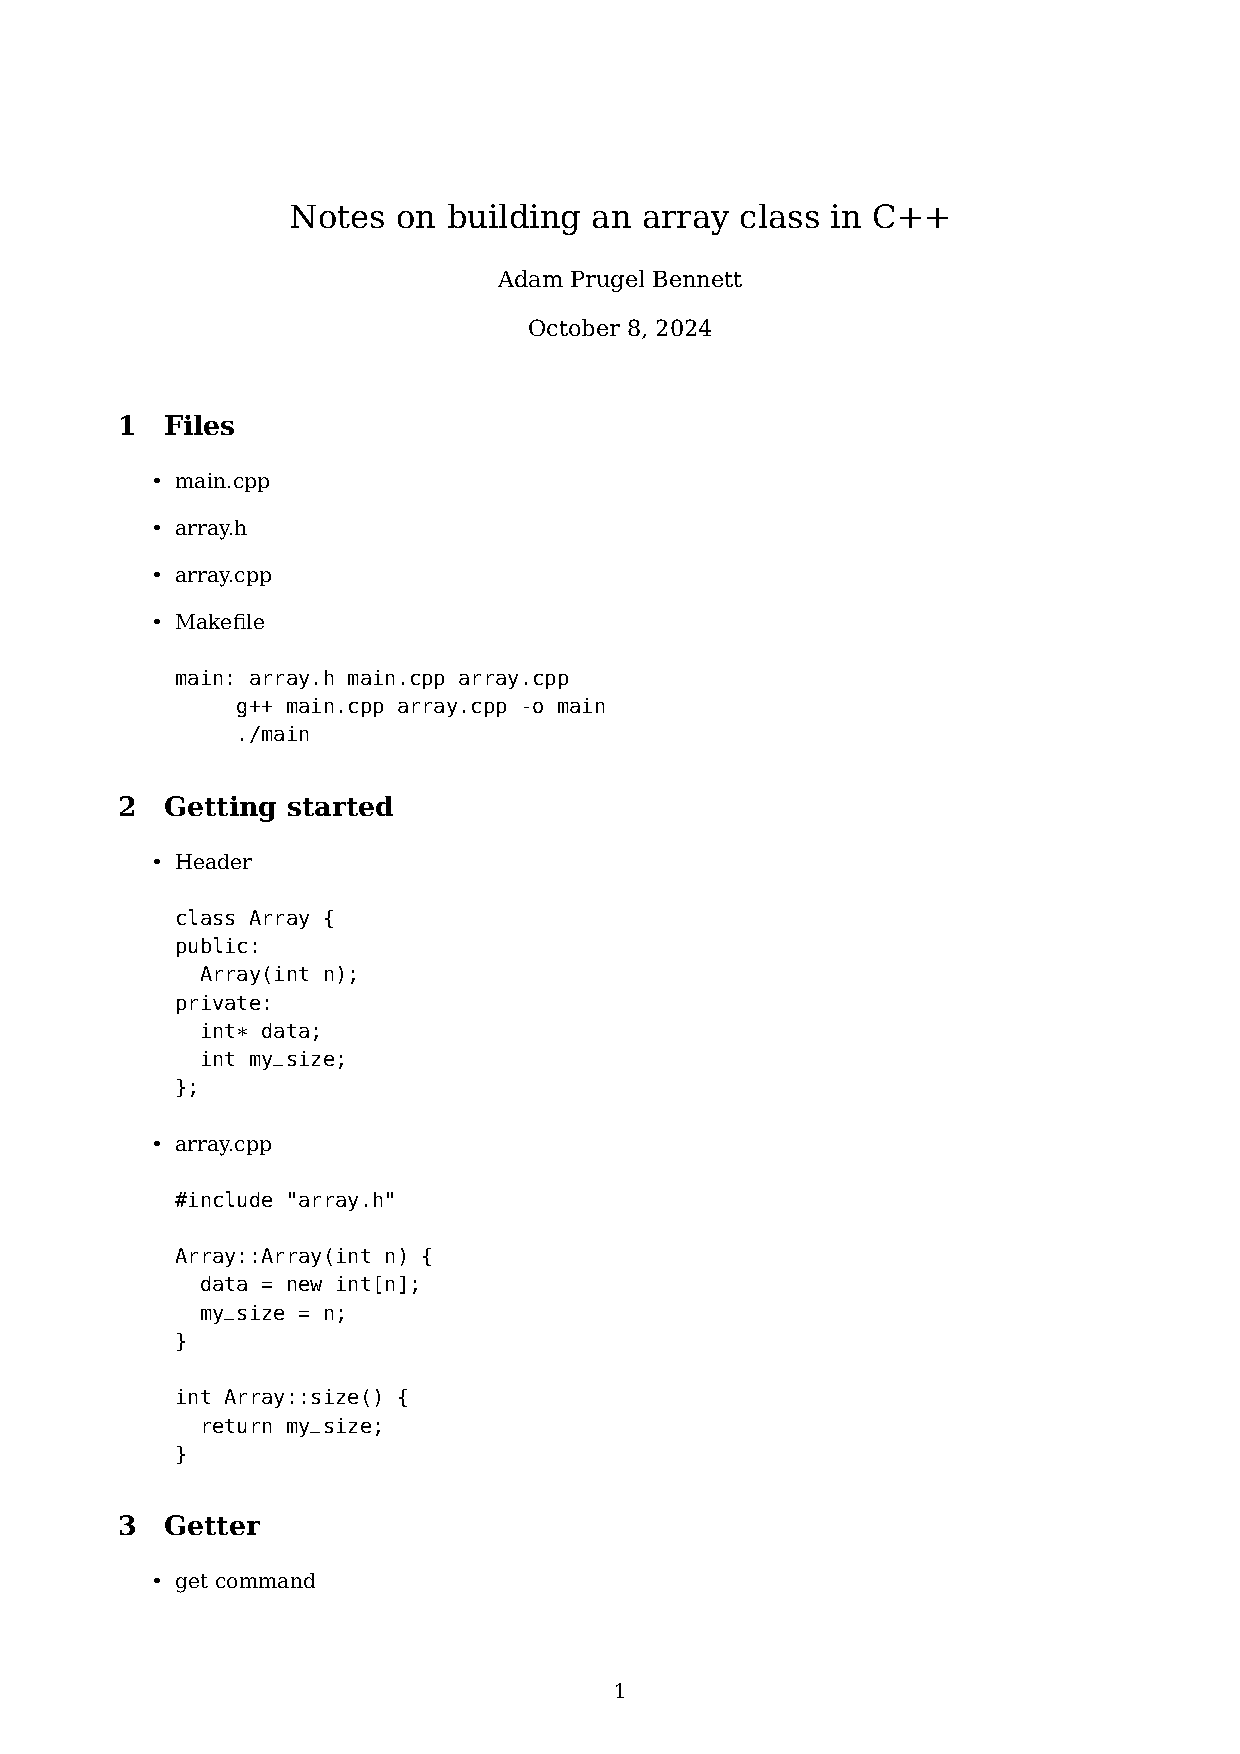
\includegraphics[height=11cm]{array}
\end{center}
\vspace*{-1cm}
\keywords{Common errors, memory leaks, templates}

%%%%%%%%%%%%%%%%%%%%%%% Next Slide %%%%%%%%%%%%%%%%%%%%%%%

\begin{slide}
  \section{Introduction}


  \begin{itemize}
  \item These are notes on the tutorial session on writing
    a resizeable array
  \item We did not get very far with them in the first lecture
  \item In this lecture we are going to make are code more solid
  \item Add some functionality
  \item Make the code generic
  \end{itemize}

\end{slide}

%%%%%%%%%%%%%%%%%%%%%%% Next Slide %%%%%%%%%%%%%%%%%%%%%%%

\begin{slide}
\section[-1]{Copy Constructor}

\begin{itemize}
\item C++ conveniently generates a copy constructor
  \begin{cpp}
    Array b(a);
  \end{cpp}
\item Unfortunately this copies the address to \jl$data$ and the
  \jl$length$
\item But his is a \textit{shallow copy} which means that both arrays
  work on the same data array
\item This would be deeply confusing.  Instead we have to write our
  own \textit{copy constructor} to do a deep copy
\end{itemize}
\begin{cpp}
Array::Array(Array& other) {
  data = new int[other.size()];
  length = other.size();
  for(int i=0; i<size(); ++i) {
    data[i] = other[i];
  }
}
\end{cpp}
\end{slide}

%%%%%%%%%%%%%%%%%%%%%%% Next Slide %%%%%%%%%%%%%%%%%%%%%%%

\begin{slide}
\section{Assignment Constructor}

\begin{itemize}
\item We can also generate a new array through assignment
  \begin{cpp}
    Array a = b;
  \end{cpp}
\item As with the copy constructor this is generated by default
\item However, it calls the copy constructor
\item If we fix the copy constructor this now works as expected
\item Almost \ldots
\end{itemize}

\end{slide}

%%%%%%%%%%%%%%%%%%%%%%% Next Slide %%%%%%%%%%%%%%%%%%%%%%%

\begin{slide}
  \section[-2]{Being Explicit}


  \begin{itemize}
  \item One oddity of C++ is that the following code compiles
    \begin{cpp}
      Array a = 4;
    \end{cpp}
    \vspace*{-1cm}
  \item We have not defined what happens when we set and array to an
    integer
  \item However, the compiler tries to make sense of this and sees
    that it can create an array on the right-hand side using the
    constructor
    \begin{cpp}
      Array(int n);
    \end{cpp}
    \vspace*{-1cm}
  \item It sees this as a way of promoting an integer to an array
  \item This isn't what most people would expect.  I expect a compile
    error
  \item To achieve this I can redefine the constructor
    \begin{cpp}
      explicit Array(int n);
    \end{cpp}
    \vspace*{-1cm}
  \end{itemize}


\end{slide}

%%%%%%%%%%%%%%%%%%%%%%% Next Slide %%%%%%%%%%%%%%%%%%%%%%%

\begin{slide}
\section{Compilers are our Friends}

\begin{itemize}
\item Compile errors are our friends\pause: they are quick to fix and
  prevent serious errors
\item One little understood strength of C++ is the compiler allows us
  to determine what changes
\item Defining the function
  \begin{cpp}
    void print(const Array&, string name);
  \end{cpp}
  \vspace*{-1cm}
  passes the array by const reference.  This is efficient.  Making it
  const means we know print won't change the reference
\item But this triggers a whole lot of consequence because print is
  only allowed to use const member functions
\end{itemize}
\end{slide}

%%%%%%%%%%%%%%%%%%%%%%% Next Slide %%%%%%%%%%%%%%%%%%%%%%%

\begin{slide}
\section[-1]{Constant consistency}

\begin{itemize}
\item At first it appears we have opened a can of works
\item We have declare lot of member functions as constant
  \begin{cpp}
    int size() const;

    int& operator[](int index);
    int operator[](int index) const;
  \end{cpp}
\item We have to declare a constant version of the access operator
\item When you first do this it seems like a lot of unnecessary work
\item But the is some satisfaction in specifying all the functions
  consistently
\item And in the long run it will prevent many bugs
\end{itemize}
\end{slide}

%%%%%%%%%%%%%%%%%%%%%%% Next Slide %%%%%%%%%%%%%%%%%%%%%%%

\begin{slide}
\section{Memory Leaks}

\begin{itemize}
\item Another ``bug'' in our code is that we are grabbing memory, but
  not giving it up
\item This can become very expensive
  \begin{cpp}
    for(int i=0; i<500000; i++) {
      Array a(10000000);
      if (i % 10000==0) {
        cout << i << endl;
        sleep(1);
      }
      cout << "Finished\n";
    }
  \end{cpp}
\item In linux I can look at memory usage using \jl=top -c $(pgrep -d',' main)$=
\end{itemize}
\end{slide}

%%%%%%%%%%%%%%%%%%%%%%% Next Slide %%%%%%%%%%%%%%%%%%%%%%%

\begin{slide}
\section{RAII}

\begin{itemize}
\item The method for preventing memory leaks is known as ``Resource
  Allocation is Initialisation''
\item This means we take the resource (in this case memory) in the
  constructor of a class
\item And give it back in the destruction
  \begin{cpp}
    Array::~Array() {
      delete[] data;
    }
  \end{cpp}
\end{itemize}
\end{slide}

%%%%%%%%%%%%%%%%%%%%%%% Next Slide %%%%%%%%%%%%%%%%%%%%%%%

\begin{slide}
\section{Make it Generic}

\begin{itemize}
\item To make an array for doubles or strings we only have to change
  the type of the data from \texttt{int} to \texttt{double} or
  \texttt{string}
\item We can write a template with \texttt{T} (or any other name we
  want to use) as representing some generic type
\item We can't compile the code as the compiler needs to know the
  type we are using
\item We would therefore have to do a global replace of \texttt{T} by
  the type we want to use and create new \texttt{array.h} and
  \texttt{array.cc} for each type of array we use
\item Fortunately the C++ compiler will do this for us
\end{itemize}

\end{slide}

%%%%%%%%%%%%%%%%%%%%%%% Next Slide %%%%%%%%%%%%%%%%%%%%%%%

\begin{slide}
\section{Template Programming}
  
\begin{PauseHighLight}
  \begin{itemize}
  \item To do this all we need to do is write
    \jl$template <typename T>$ in front of any class or function that
    uses a generic type
  \item These need to be included in the header file
  \item In the main code to ask for an array of type \texttt{string},
    for example, we write
    \begin{cpp}
      Array<string> string_array;
    \end{cpp}
  \item The compiler invisibly creates the code for this class, but
    replacing the template variable by \texttt{string}
  \end{itemize}
\end{PauseHighLight}

\end{slide}

%%%%%%%%%%%%%%%%%%%%%%% Next Slide %%%%%%%%%%%%%%%%%%%%%%%

\begin{slide}
\section[-2]{Template Code Example}

\begin{cpp}
template <typename T>
class Array {
private:
  T *data;
  unsigned length;
public:
  explicit Array(int n);
  Array(const Array& other);
  ~Array();
  T& operator[](unsigned index);
  T operator[](unsigned index) const;
  unsigned size() const;
};

template <typename T>
Array<T>::Array(int n) {
  data = new T[n];
  length = n;
}
\end{cpp}
\end{slide}
